\documentclass[12pt, letterpaper]{article}

\usepackage[T1]{fontenc}

\usepackage{polski}
\usepackage[utf8]{inputenc}
\usepackage[polish]{babel}
\usepackage{wrapfig}
\usepackage{comment}
\usepackage{lipsum}
\usepackage{amsmath}
\newcommand{\Mod}[1]{\ \mathrm{mod}\ #1}
 
\usepackage[
backend=biber,
style=numeric,
sorting=ynt
]{biblatex}
\addbibresource{bib.bib}

\usepackage{amsmath} % Advanced math typesetting
\usepackage{graphicx} % Add pictures to your document
\usepackage[export]{adjustbox}

\begin{document}

\begin{figure}[t]
	\centering
	
\includegraphics[width = 0.9\textwidth]{{pics/agh.png}}
\end{figure}

\author{Konrad Rzońca} 
\title{\Huge Algorytm Shor'a} 
\date{\normalsize\today{}} 

\maketitle{} 
\newpage{}

\tableofcontents{} 
\newpage{}




\section{Wstęp} 

Aby zrozumieć i skutecznie omówić działanie algorytmu Shor'a na przykładzie układu elektronicznego zacznę od omówienia działania komputera kwantowego, używanych w nim bramek i idei stojącej za algorytmem.

\subsection{Komputer kwantowy}

\subsubsection{Qubity}

W taki sam sposób jak tradycyjne komputery operują na bitach, komputery kwantowe operują na qubitach, są to zazwyczaj pojedyńcze elektrony lub protony.\cite{qubit}

Spin cząstki w polu magnetycznym, w momencie pomiaru, może przyjmować tylko dwa stany - zgodnie z polem w którym się znajduje czyli spin-up state, lub przeciwnie - spin-downstate. 
Jednak w większości przypadków znajdują się one w stanie superpozycji - ich stan jest niemożliwy do stwierdzenia, aż do dokonania pomiarów, możemy go jedynie określać z pewnym prawdopodobieństwem. \cite{spin}

Dodatkową własnością takich cząstek, jest to, że mogą być ze sobą w stanie związania (quantum entanglement), jest to zjawisko jeszcze niewyjaśnione przez fizykę, pomiar jednej ze związanych ze sobą cząstek determinuje stan tej drugiej - zależnie od splątania będzie miała ona stan ten sam lub przeciwny do cząstki którą mierzymy \cite{qubit}

\subsubsection{Stan qubita}

Stan każdego qubita w układzie określić możemy jako $ a|0\rangle + b|1\rangle, a,b \in C  $, gdzie $ a^2 + b^2 = 1 $.
W praktyce oznacza to, że prawdopodobieństwo, że po pomiarze qubit przyjmie stan 0 z prawdopodobieństwem $a^2$, stan 1 $b^2$. 

\newpage
\subsubsection{Stan komputera kwantowego}

Stan całej maszyny określa się jako przestrzeń Hilberta w której $|0\rangle$ oraz $|1\rangle$ są jej wektorami bazowymi. \cite{pdf} Aktualny stan maszyny jest punktem w $2^n$ wymiarowej przestrzeni wektorowej. Kombinacje stanu dwóch systemów kwantowych możemy określić jako tensor z argumentów podsystemów, zatem stan układu dwoje qubitów: $|A\rangle = a_0|0\rangle + a_1|1\rangle$ oraz $|B\rangle = b_0|0\rangle + b_1|1\rangle$ możemy rozpisać jako: 
\[ |A\rangle|B\rangle = 
\left(\!
\begin{array}{c}
      a_1 \\
      a_2
    \end{array}
  \!\right)
  \otimes
  \left(\!
\begin{array}{c}
      b_1 \\
      b_2
    \end{array}
  \!\right) = 
  \left(\! 
\begin{array}{c}
      a_1b_1 \\
      a_1b_2 \\
      a_2b_1 \\
      a_2b_2 \\
    \end{array} 
  \!\right)
  \] 
Stan takiego układu możemy zapisać jako $|A,B\rangle$.

Późniejsze operacje na qubitach zazwyczaj są opisywane jako macierze $2^n \times 2^n$, przykładowo reprezentacja macierzowa M =\[
 \begin{bmatrix}
  0 & 1 & 0 & 0 \\
  i & i & 0 & 0 \\
  0 & 1 & i & 1 \\
  1 & 1 & 1 & 1
 \end{bmatrix}
\] 
oznaczałaby, że \newline
$M|0,0\rangle = |0,1\rangle$, czyli prawdopodobieństwo układu 0,0 byłoby po przejściu równe
prawdobodobieństwu układu 0,1 przed przejściem \newline 
$M|0,1\rangle = i|0,0\rangle + i|0,1\rangle$ itd. \newline
Zauważmy, że bramka M nie byłaby fizycznie możliwa do zrealizowania, ponieważ 
$ M|0,0\rangle^2 + M|0,1\rangle^2 + M|1,0\rangle^2 + M|1,1\rangle^2$ != 1 \newline (chociażby dlatego, że dla układu wejściowego spełniającego warunek z kwadratami $M|1,1\rangle^2$
musiałoby się równać 1 a $ M|0,0\rangle^2 + M|0,1\rangle^2 + M|1,0\rangle^2 > 0)$ 


\newpage


\subsubsection{Sfera Bloch'a}


\begin{figure}[h] 
    \centering
    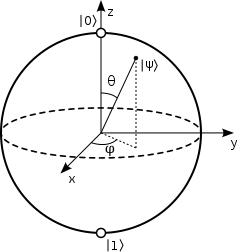
\includegraphics[width = 0.5\textwidth]{{pics/bloch.png}}
    \caption{\label{fig:bloch} Sfera Bloch'a}
\end{figure}

Jednym z bardziej popularnych sposobów przedstawiania stanu qubita jest tzw. sfera Bloch'a.
Rezprezentuje ona stan pure pojedyńczego stanu kwantowego drugiego poziomu który możemy zapisać w postaci \[ |\psi\rangle = a|0\rangle + b|1\rangle \]
Stan ten, tak jak było to opisane w poprzednich podpunktach, musi spełniać warunek $a^2 + b^2 = 1$. Rozważmy liczbę zespoloną z która będzie reprezentacją stanu naszego qubita \[z = x + iy, x,y \in R\]
Liczba z musi spełniać nasz pierwotny warunek zatem $|z|^2 = 1$, rozpisując ją dalej uzyskujemy $ z*z = (x + iy)^2 = x^2 + y^2$, jest to równanie koła w centrum w (0,0).\cite{bloch}
\newpage
Przechodząc na współrzędne sferyczne i biorąc pod uwagę, ze promień sfery którą rozważamy wynosi 1 uzyskujemy $ z = r(\cos\theta + i\sin\theta) = re^{i\theta} = e^{i\theta}$
Pozostawia nas to zatem z jednym stopniem swobody, reprezentacja fizyczna z-eta to po prostu stan naszego spinu, dla z = 1 spin będzie górny (spin-up - $|0\rangle$, czyli a = 1), natomiast kiedy z = -1 to spin będzie dolny.\\\\
Wracając do naszych parametrów a, b je reprezentujemy kolejno jako $r_ae^{i\phi_a}$ i $r_be^{i\phi_b}$, nie potrzebujemy się wgłębiać bardziej w matematykę, co jest istotne to intuicja związana z tym układem która jest potem przydatna w rozumieniu bramek Pauliego.





\newpage

\subsection{Podstawowe bramki}
\subsubsection{Hadamard gate}
Podstawową intuicją stojącą za bramkami Hadamarda jest to, że pozwalają nam przejść w stan super pozycji dwóch stanów,
oraz z niego wyjść. Bramki Hadamarda wykorzystuje się głównie, aby generować losowe stany wyjścia, sytuacja jednak staje się ciekawsza
kiedy połączymy je z innymi bramkami, możemy wtedy wykonywać obliczenia na wszystkich możliwych wejściach jednocześnie, 
następnym ciekawym faktem jest, że po dwuktrotnym przejściu przez bramkę Hadamarda otrzymamy identyczność. \cite{hadamard}

\begin{figure}[h]
	\centering
	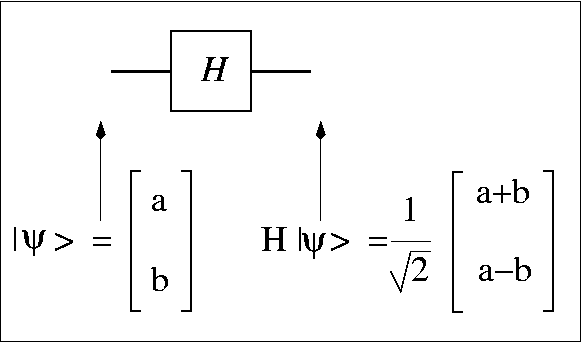
\includegraphics[width = 0.7\textwidth]{{pics/hadamard.png}}
	\cite{hadpic}
\end{figure} 


	\[ |0\rangle \to \frac{|0\rangle + |1\rangle}{\sqrt2} \]   \[  |1\rangle \to \frac{|0\rangle - |1\rangle}{\sqrt2} \]
\normalsize

Bramkę Hadamarda możemy przedstawić również w reprezentacji \\  macierzowej
\[ H = \frac{1}{\sqrt2}
\begin{bmatrix}
  1 & 1 \\
  1 & -1
 \end{bmatrix}
\]



\newpage
\subsubsection{Pauli-X gate czyli kwantowa bramka NOT}

Bramka X jest odpowiednikiem kwantowym klasycznej bramki NOT - zmienia stan qubita na przeciwny. Obraca ona nasz układ o $\pi$ rad w okół osi x w układzie sfery Bloch'a\cite{bramki}

\begin{figure}[h]
	\centering
	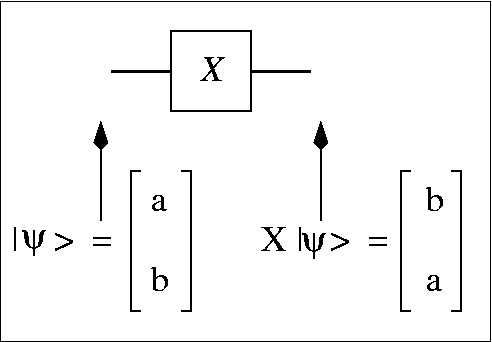
\includegraphics[width = 0.7\textwidth]{{pics/X.png}}
	\cite{hadpic}
\end{figure} 



Bramka X przedstawiona w reprezentacji macierzowej to: 
\[ X = 
\begin{bmatrix}
  0 & 1 \\
  1 & 0
 \end{bmatrix}
\]
natomiast w układach bramki NOT często są przedstawiane również jako 

\begin{figure}[h]
	\centering
	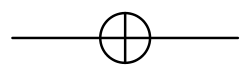
\includegraphics[width = 0.3\textwidth]{{pics/circuitNOT.png}}
	\cite{bramki}
\end{figure} 


Mapuje ona wartość $|0\rangle$ do $|1\rangle$ i na odwrót.
X(X(A)) = A

\newpage
\subsubsection{Pauli-Y gate}
Ta bramka nie ma odpowiednika w układach klasycznych, tak jak bramka X obraca układ na osi x o $\pi$ radianów, tak bramka Y robi to dla osi y\cite{bramki}
\begin{figure}[h]
	\centering
	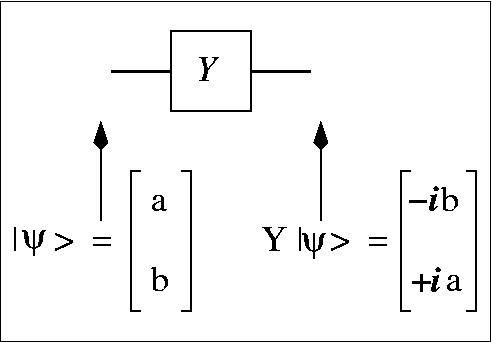
\includegraphics[width = 0.7\textwidth]{{pics/Y.png}}
	\cite{hadpic}
\end{figure} 



Bramka Y przedstawiona w reprezentacji macierzowej to: 
\[ Y = 
\begin{bmatrix}
  0 & -i \\
  i & 0
 \end{bmatrix}
\]
Możemy łatwo obliczyć, że Y(Y(A)) = A, co jest zresztą bardzo intuicyjne - obrót w okół którejkolwiek z osi układu współrzędnych o łączne 2$\pi$ radianów wraca nasz układ do pozycji startowej 

\newpage
\subsubsection{Pauli-Z gate}
Analogicznie, bramka Z obraca układ o $\pi$ radianów na osi z.\cite{bramki}



\begin{figure}[h]
	\centering
	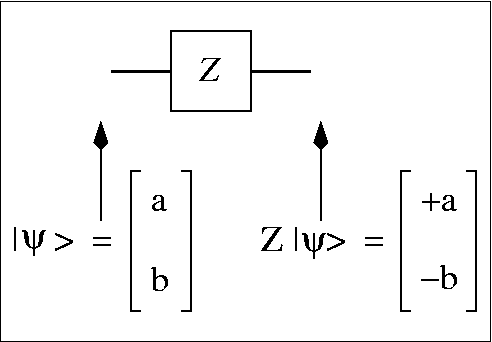
\includegraphics[width = 0.7\textwidth]{{pics/Z.png}}
	\cite{hadpic}
\end{figure} 
Z(Z(A)) = A

Bramka Z przedstawiona w reprezentacji macierzowej to: 
\[ Z = 
\begin{bmatrix}
  1 & 0 \\
  0 & -1
 \end{bmatrix}
\]
Z(Z(A)) = A

\newpage
\subsubsection{CNOT gate}
Bramka CNOT (controled NOT) do działania potrzebuje przynajmniej dwóch qubitów, domyślnie zmienia ona stan qubita na przeciwny kiedy qubit kontrolny jest równy 1\cite{bramki}

Schemat bramki CNOT kontrolowanej przez qubit to
\begin{figure}[h]
	\centering
	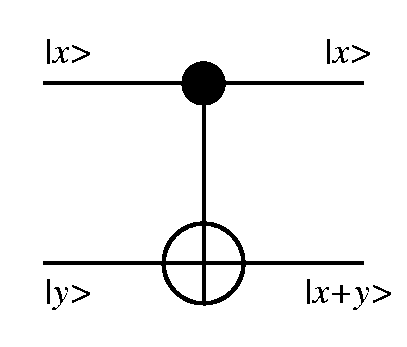
\includegraphics[width = 0.3\textwidth]{{pics/cnot.png}}
	\cite{hadpic}
\end{figure} 

Schemat i działanie wszystkich bramek kontrolowanych jest analogiczny: są oznaczane jak bramka kontrolowana dopięta do qubita kontrolującego jej działanie. Nie będę w związku z tym omawiał wersji kontrolowanych wszystkich przedstawionych bramek.

Powyższa bramka CNOT przedstawiona w reprezentacji macierzowej to: 
\[ CNOTx = 
 \begin{bmatrix}
  1 & 0 & 0 & 0 \\
  0 & 1 & 0 & 0 \\
  0 & 0 & 0 & 1 \\
  0 & 0 & 1 & 0
 \end{bmatrix}
\] 
$CNOTx|0,0\rangle = |0,0\rangle$ \newline
$CNOTx|0,1\rangle = |0,1\rangle$ \newline
$CNOTx|1,0\rangle = |1,1\rangle$ \newline
$CNOTx|1,1\rangle = |1,0\rangle$ \newline
Widzimy zatem, że dla qubita kontrolnego x równego 1 bramka wykonuje operację NOT na wejściu y, w systemie binarnym możemy po prostu zapisać, że y = x + y \newline
Pamiętajmy, że współczynniki przy poszczególnych qubitach opisane w 1.1.2 to nie ich wartość, ale prawdopodobieństwo, że ją przybiorą, w trakcie pomiaru qubit zawsze jest równy 0 lub 1 - stan wyjściowy bramki przybiera wartość jednoznaczną.




\newpage
\subsubsection{S gate}
Bramka S nazywana również SWAP służy do zamiany stanu dwóch bitów.\cite{bramki}

\begin{figure}[h]
	\centering
	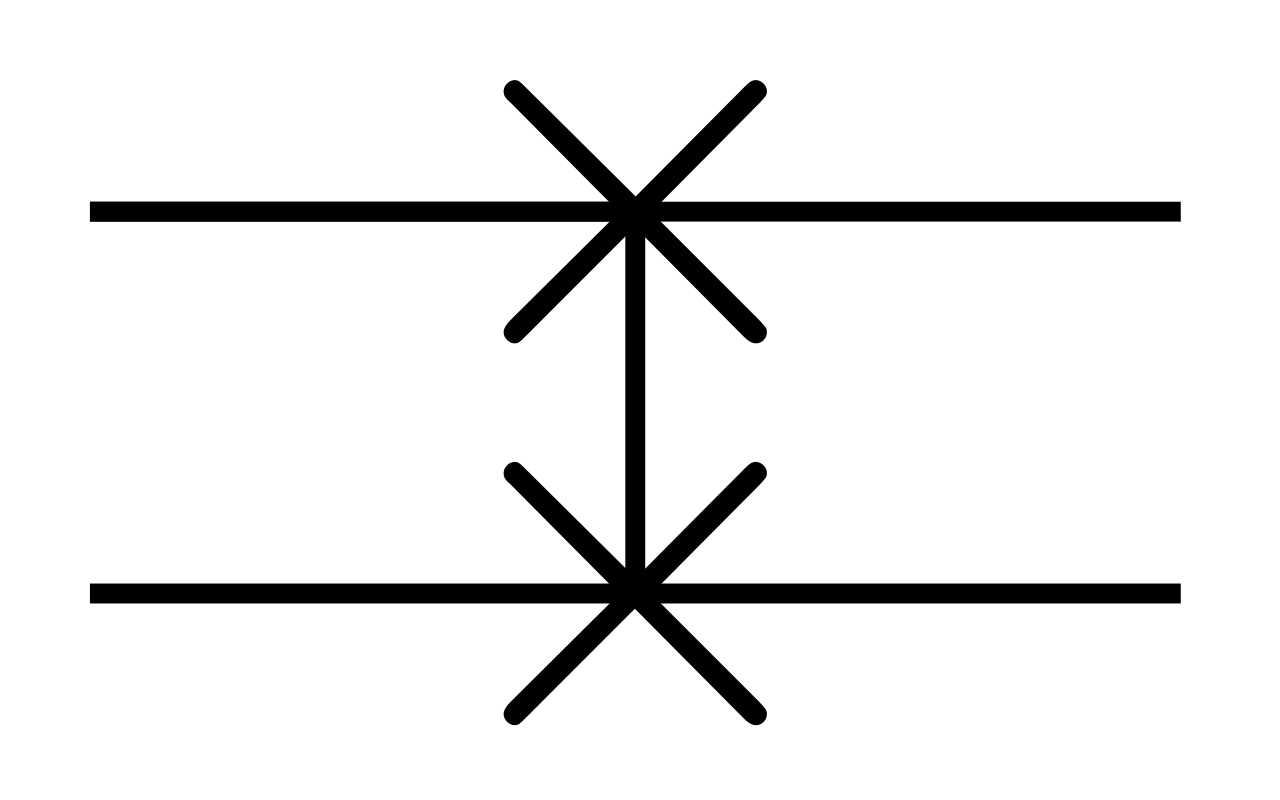
\includegraphics[width = 0.4\textwidth]{{pics/S.png}}
	\cite{bramki}
\end{figure} 

Bramka S przedstawiona w reprezentacji macierzowej to: 
\[ SWAP = 
 \begin{bmatrix}
  1 & 0 & 0 & 0 \\
  0 & 0 & 1 & 0 \\
  0 & 1 & 0 & 0 \\
  0 & 0 & 0 & 1
 \end{bmatrix}
\] 
$SWAP|0,0\rangle = |0,0\rangle$ \newline
$SWAP|0,1\rangle = |1,0\rangle$ \newline
$SWAP|1,0\rangle = |0,1\rangle$ \newline
$SWAP|1,1\rangle = |1,1\rangle$ \newline
Łatwo wywnioskować, że S(S(A)) = A

\newpage
\subsubsection{T gate}
Bramka T to jak bramka Z ale obracamy nie o $\pi$ a $\frac{\pi}{4}$

\begin{figure}[h]
	\centering
	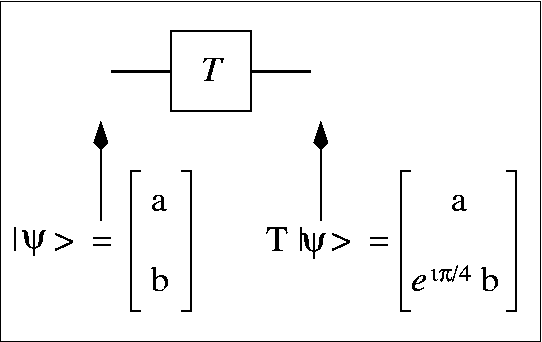
\includegraphics[width = 0.7\textwidth]{{pics/T.png}}
	\cite{bramki}
\end{figure} 

Bramka T przedstawiona w reprezentacji macierzowej to: 
\[ T = 
\begin{bmatrix}
  1 & 0 \\
  0 & e^{i\pi/4}
 \end{bmatrix}
\]
$T|0\rangle = |0\rangle$ \newline
$T|1\rangle = e^{i\pi/4}|1\rangle$ \newline

T(T(T(T(T(T(T(T(A)))))))) = A - po 8 krotnym użyciu bramki T qubit wraca do stanu pierwotnego: $\frac{\pi}{4}*8 = 2\pi$, spotkałem się również w podanych źródłach z bramką S(A) = T(T(A)), zatem SWAP będziemy zawsze oznaczać jako SWAP.

Jeżeli chodzi o intuicje stojącą za tym, że całkowite prawdopodobieństwo będzie nadal równe jeden wróćmy do naszej reprezentacji układu w sferze Bloch'a b = $r_be^{i\phi_b}$, po pomnożeniu przez $e^{i\pi/4}$, $(|b'|)^2$ = $(|r_be^{i\phi_b}*e^{i\pi/4}|)^2 = b^2 * |e^{i\pi/2}| = b^2$ zatem równanie jest zachowane, bardziej ogólnie obracając w okół z zawsze zachowamy wartość modułu.   
\newpage




\section{Opis ogólnego działania algorytmu Shor'a }
\subsection {Zasada działania algorytmu Shor'a} 
Algorytm Shor'a jest algorytmem służącym do szukania rozkładu liczby naturalnej na dwie liczby pierwsze, wiemy, że każda liczba ma dokładnie jeden taki rozkład.\cite{shoropis}

\begin{figure}[h] 
    \centering
    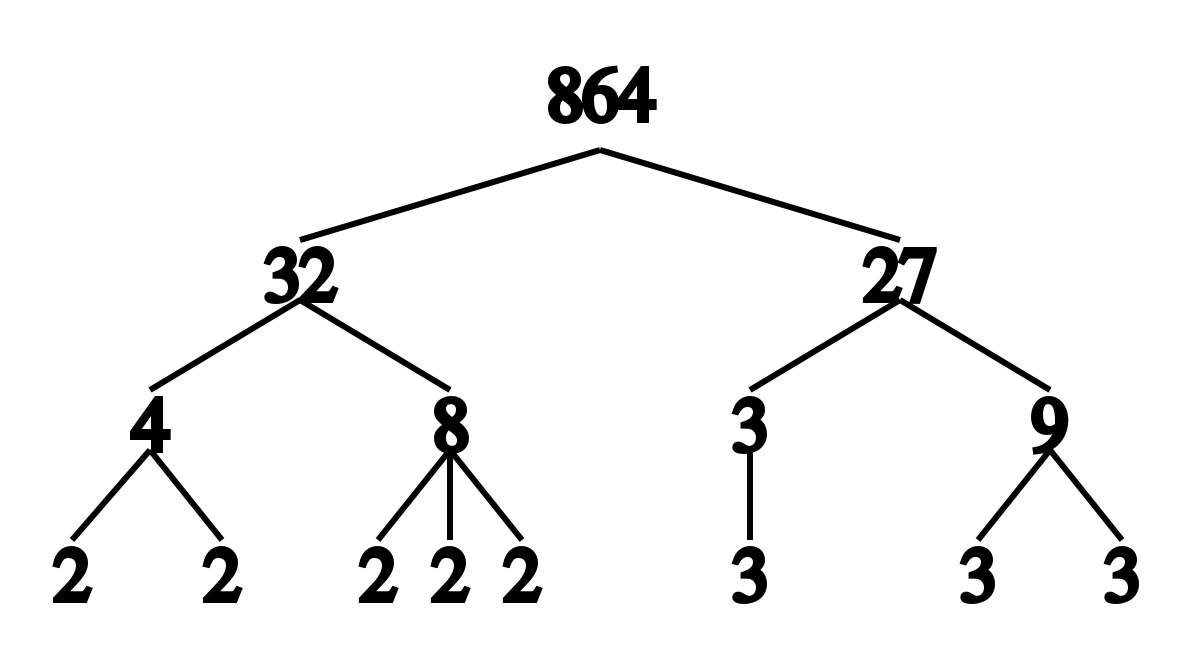
\includegraphics[width = 1\textwidth]{{pics/prime.png}}
    \caption{\label{fig:bloch} rozkład 864}
\end{figure}



Dzięki narzędziom matematycznym możemy ograniczyć problem szukania rozkładu liczby to problemu szukania okresu pewnego ciągu elementów, weźmy sobie np. ciąg którego n-ty wyraz to$x(n) = 2^n$
\[2, 4, 8, 16, 32, 64, 128, 256 ...\]
Teraz, weźmy zamiast tego ciąg $x(n) = 2^n \mod 15$, czyli reszty z dzielenia przez 15 każdego z wyrazów wyższego ciągu, co otrzymamy to
\[2, 4, 8, 1, 2, 4, 8, 1, 2, 4, 8, 1, 2, 4, 8, 1 ...\]
\newpage
Jest to ciąg okresowy o okresie równym 4. 
Euler odkrył, że jeżeli, weźmiemy dwie liczby pierwsze p i q, $m = p*q$, oraz jakieś x niepodzielne ani przez q ani p (w naszym wyższym przykładzie 2) to ciąg $a_n = x^n \mod m$
\[x \Mod{m}, x^2 \Mod{m}, x^3 \Mod{m}, ...\]
posiada okres który jest dzielnikiem (p - 1)(q - 1).
Dla naszego przykładu p = 3, q = 5, m = 15, x = 2, zatem zgadza się, 4 dzieli 2*4 = 8.
Daje nam to jeden z dzielników (p-1)(q-1), po wypróbowaniu wystarczająco wielu x-ów uzyskujemy cały iloczyn co z kolei daje nam potem możliwość wiliczenia samych p i q.

Jest to niewykonywalne w tradycyjnym systemie komputerowym ponieważ sam okres może wynosić prawie m, a jest tylko jednym z kroków w działaniu naszego algorytmu, przy dużych liczbach jak te używane do szyfowania RSA ma to bardzo dużą złożoność, jednak układy kwantowe pozwalają nam ją obejść.
\newpage
Sam algorytm Shor'a działa w następujących krokach: 


\begin{enumerate}
\item Bierzemy losową liczbę naturalną k taką, że k < m. Obliczamy (ze złożonością wielomianową np. algorytmem Euklidesa) największy wspólny dzielnik m i k (gcd(m,k)), 
jeżeli gcd(m,k) $\ne$ 1, to znaleźliśmy dzielnik m i jest nim k, kończymy. jeżeli jednak gcd = 1 kontynuujemy dalej.

\item Znajdujemy okres P \[ k \Mod{m}, k^2 \Mod{m}, k^3 \Mod{m}, ...\]

\item Dla P nieparzystego wracamy na początek, dla parzystego kontynuujemy

\item $(k^{P/2} - 1)(k^{P/2} + 1) = k^P - 1$, teraz zauważmy, że tak jak w przykładzie gdzie k = 2, $k^P \Mod{m} = 1$, wracając jeszcze raz do przykładu   
\[2, 4, 8, 1, 2, 4, 8, 1, 2, 4, 8, 1, 2, 4, 8, 1 ...\]
$2^4 \Mod{15} = 16 \Mod{15} = 1$, ostatni wyraz w pojedyńczym okresie tego ciągu to zawsze jeden dla dowolnych k,m naturalnych, będzie on miał numer P stąd ten rachunek.\\
Dalej, wiemy już, że $(k^P - 1) \Mod{m} = 0$, jeżeli $(k^{P/2} + 1) \Mod{m} = 0$ to wracamy do początku, inaczej kontynuujemy

\item Liczymy d = $gcd(k^{P/2} - 1, m)$, dla $(k^{P/2} + 1) \Mod{m} \ne 0$ potrafimy wykazać, że d jest nietrywialnym ($\ne 1, m$)dzielnikiem m-a. \\Zwracamy d. W ten sposób możemy wyznaczyć dzielniki m-a, jeżeli to dwie liczby pierwsze tak jak w RSA to je znajdziemy.

\end{enumerate}




















\newpage
\subsection {Implementacja algorytmu Shor'a na układzie kwantowym} 

Kwantowy algorytm shor'a do działania potrzebuje dwóch rejestrów kwantowych. Na początku pierwszy rejestr musi znaleźć liczbę $q = 2^s, s \in N$ która spełni warunek $n^2 \leq q < 2n^2$, gdzie n to rozkładana liczba, zauważmy, że zawsze istnieje taka liczba. Następnie należy wykonać następujące kroki\cite{pdf}

\begin{enumerate}
\item \textsl{Inicjalizacja}: Umieszczamy pierwszy rejestr w superpozycji 
\[\frac{1}{\sqrt{q}}\sum_{a=0}^{q-1}|a\rangle|0\rangle\] 
Zauważmy, że ${0,1,\sqrt{2}, \sqrt{3} ... \sqrt{q-1}}$ to wszytskie możliwe dzielniki piersze n-a co wynika z warunku jaki narzuciliśmy na q.

\item \textsl{Obliczenia}: Wybieramy losowe x i liczymy w drugim rejestrze $x^a$
\[\frac{1}{\sqrt{q}}\sum_{a=0}^{q-1}|a\rangle|x^a\rangle\] 
 
Teraz przykład, stan maszyny kwantowej  
\[\frac{1}{\sqrt{7}}\sum_{k=0}^{4}|5k\rangle\]
możemy zapisać jako $\frac{1}{\sqrt{7}}|00000\rangle + \frac{1}{\sqrt{7}}|00101\rangle + \frac{1}{\sqrt{7}}|01010\rangle + \frac{1}{\sqrt{7}}|01111\rangle + \frac{1}{\sqrt{7}}|11001\rangle$, przypisuje on  $\frac{1}{\sqrt{7}}$ decymalnie stanom 0,5,10,15,20. Inne stany nie będą posiadały wartości, zatem posiada on okres równy 5. Po transformacie Fouriera uzyskalibyśmy zatem 5 lokalnych maksimów w rozkładzie stanu tego układu.\cite{furier} 

\begin{minipage}{0.5\textwidth}
      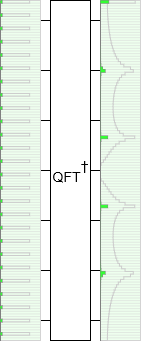
\includegraphics[width = 0.6\textwidth]{{pics/furier.png}}\cite{furier}
    \end{minipage}
 \begin{minipage}{0.5\textwidth}
     Na tym obrazku maksima reprezenotwane są przez zielone znaczniki. ransformatę Fouriera będziemy wykonywać w kroku następnym na pierwszym rejestrze.
    \end{minipage}

Wracamy do naszego układu
\LARGE \[\frac{1}{\sqrt{q}}\sum_{a=0}^{q-1}|a\rangle|x^a\rangle\] \normalsize


\item \textsl{Transformata Fouriera}: Za pomocą bramek Hadamarda i bramek zmiany fazy jesteśmy w stanie przeprowadzać transformaty Fouriera w naszych układach, po dokonaniu jej na pierwszym rejestrze stan naszej maszyny możemy wyrazić jako:

\LARGE \[\frac{1}{q}\sum_{a=0}^{q-1}\sum_{c=0}^{q-1}(e^{2\pi iac/q})|c\rangle|x^a\rangle\] \normalsize

\newpage
\item \textsl{Obserwacje}: W naszej sumie znajdzie się okres którego szukamy, mianowicie 
jeżeli weźmiemy jakieś $x^k$, i weźmiemy te części sumy po a w których $x^a\, \equiv\, x^k$ mod n, do dla danego c prawdopodobieństwo, że maszyna znajdzie się w stanie $|c\rangle|x^k\rangle$
możemy określić jako

\LARGE \[\Bigg|\,\,\frac{1}{q}\sum_{a: \,\,x^a\, \equiv\, x^k}^{q-1}(e^{2\pi iac/q})\,\,\Bigg|^2\] \normalsize
k wybieramy takie, że 0 $\le$ k < r, a r to najmniejsza liczba naturalna spełniająca równanie 
 $x^r \equiv$ 1 mod n 


\item \textsl{Continued Fraction Expansion}: Jeżeli istnieje takie d, że 
\[\frac{-r}{2} \le dq - rc \le \frac{r}{2} \]
to prawdopodobieństwo wystąpienia $|c,x^k\rangle$ jest większe niż 1/3$r^2$, następnie d/r może być otrzymane przez zaokrąglenie c/q. r to prawdopodobny okres Q.


\newpage




\end{enumerate}







\newpage
\section{Działanie algorytmu Shor'a na przykładzie rozkładu liczby 21 w konkretnym obwodzie kwantowym za pomocą narzędzia Quirk}


Posługiwać się będę krokami z rozdziału 2.1 i narzędziem Quirk, a konkretnie zaproponowanym w nim obwodzie to liczenia okresu P. Jest to jedynie obwód symulacyjny i wiele dość skomplikowanych układów upraszcza, jednak pomaga on przedstawić samą ideę.

Schemat proponowany przez Quirka wygląda następująco


\begin{figure}[h] 
    \centering
    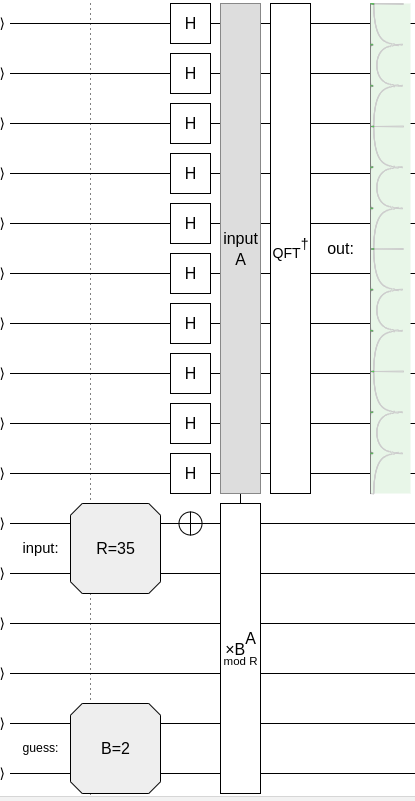
\includegraphics[width = 0.5\textwidth]{{pics/q1.png}}
    \cite{quirk}
\end{figure}

Najpierw inicjalizujemy 10 stanów nieoznaczonych za pomocą bramek Hadamarda, $21^2 = 441$, 
$441 < 512 < 882$, potrzebujemy zatem 9 bramek więc 10 wyrzucam z układu.
Następnie liczymy $k^r mod N$, gdzie k to wybrana w kroku pierwszym liczba, N to liczba której rozkładu szukamy, a r to będą wszystkie liczby z zakresu od 0 do 512, na raz.
Następnie za pomocą transformaty Fouriera zczytujemy okres, przejdźmy do praktyki.\\
21 wybrałem losowo i robię to pierwszy raz na quirku.

\begin{enumerate}

\item Za k biorę 2, spełnia warunki

\item Okres jaki wskazał Quirk to 6, obrazek z pomiaru na następnej stronie, należy policzyć zielone kreski na transformacie Fouriera odpowiadające maksimom lokalnym.

\item 6 jest parzyste, kontynuujemy

\item 9 mod 21 to nie zero więc przechodzimy do ostatniego kroku

\item Liczymy d = gcd(7, 21) = 7, zgadza się ! 21/7 = 3, zatem algorytm działa

\end{enumerate}
\newpage

\begin{figure}[h] 
    \centering
    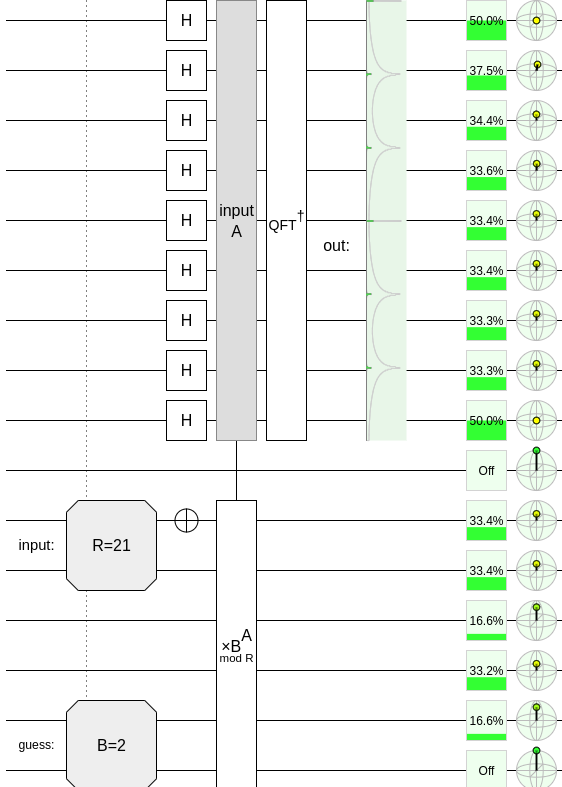
\includegraphics[width = 0.75\textwidth]{{pics/q3.png}}

\end{figure}








\newpage

\printbibliography
\end{document}


